% ------------------------------------------------------
\chapter{Felhasználói dokumentáció}
\label{ch:user}
% ------------------------------------------------------

\section{A megoldott probléma}

A készített programmal harmadfokú Bézier-felületek jeleníthetők meg. A Bézier-felületeket egy kontrollpont-háló definiálja. A felület pontjait a kontrollpontok speciális súlyozott átlagaként kapjuk. A felület modellezés szempontjából legfontosabb tulajdonsága, hogy a kontrollpontoknak a pont környezetében van leginkább hatása, így a felület a kontrollpont-hálón keresztül intuitívan manipulálható.

Ha a felülethez árnyékokat is szeretnénk számítani, akkor általában valamilyen sugárkövetési algoritmust használunk. A programban az ún. sphere trace sugárkövető algoritmust használtam. Ennek megvalósításához szükség van a felületet határoló dobozon belül minden pontban a felület távolságára vagy annak egy \emph{alsó} közelítésére. Ezt nevezzük távolságfüggvénynek. A távolságfüggvényt egy diszkrét rácson kiértékelem, majd textúrában eltárolom. Ezt nevezzük távolságmezőnek. A távolságmezőt elég a program elején kiszámítani, mert ha a felület nem változik, akkor minden képkocka kirajzolásakor újrahasználható.

A távolságmező generálására több különböző algoritmust is implementáltam. A program segítségével ezeknek a módszereknek a paramétereivel lehet kísérletezni, illetve az egyes módszereket össze lehet hasonlítani.


\section{A felhasznált módszerek}

\subsection{Tesszelláció}
A legelső megjelenítési mód a felület háromszögekkel való közelítése. A tesszelláció vagy háromszögelés során a cél úgy lefedni háromszögekkel a felületet, hogy annak részletei ne vesszenek el. Ez egyben a leggyakrabban használt modellezési módszer is. A videókártyák hardveresen támogatják háromszögek raszterizációját, így ez a módszer nagyon gyors. A többi módszer helyességét a háromszögekkel tesszellált közelítéssel fogom ellenőrizni. Ha függvények grafikonjait háromszögeljük, általában egyenletes felosztást veszünk a parmétertérben. A függvényértéket a harmadik koordináta reprezentálja.
\begin{figure}[H]
	\centering
	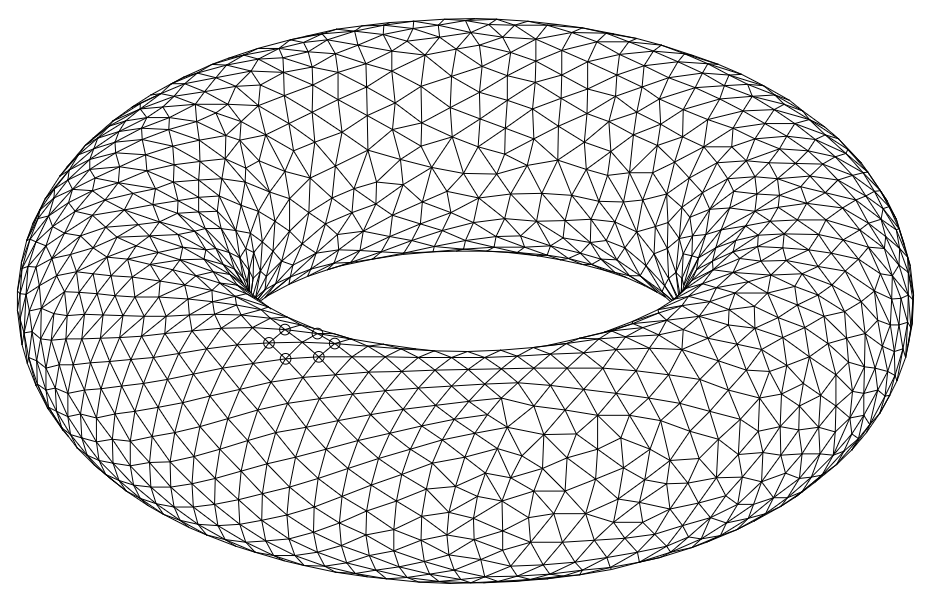
\includegraphics[width=0.4\textwidth]{tess_torus}
	\hspace{5pt}
	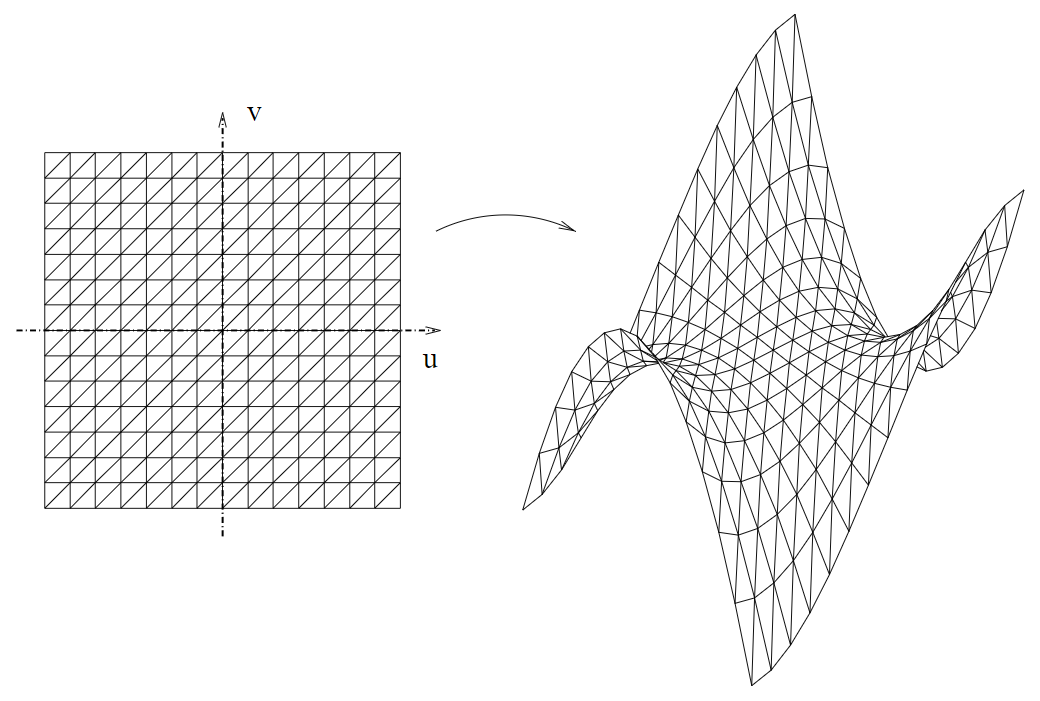
\includegraphics[width=0.4\textwidth]{tess_graph.png}
	\caption{Tórusz és függvénygrafikon háromszögelése. Forrás: \href{https://www.wikiwand.com/en/Surface_triangulation}{wikiwand.com}}
\end{figure}

\subsection{Sugárkövetés motivációja}
A sugárkövetés mindenképpen költségesebb művelet, mint a raszterizáció, hiszen visszaverődéseket, törést és árnyéksugarakat is számítunk a jobb eredmény érdekében. Ha a fotorealisztikus eredmény a cél, akkor viszont mindenképpen sugárkövetést használunk, és a cél az extra számítási költségek csökkentése, a sugárkövetés felgyorsítása. 
\begin{figure}[H]
	\centering
	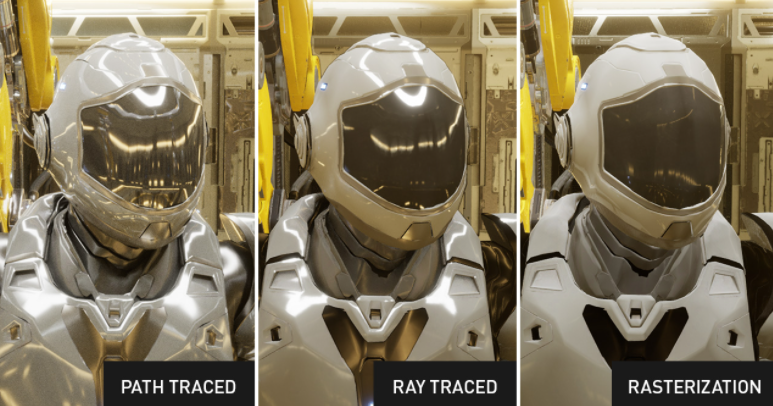
\includegraphics[width=0.7\textwidth]{pt-rt-raster}
	\caption{Megjelenítési módok összehasonlítása. Forrás: \href{https://blogs.nvidia.com/blog/2022/03/23/what-is-path-tracing/}{blogs.nvidia.com}}
\end{figure}


\section{Távolságmező-számítás}

\subsection{Lipschitz-módszer}
A Lipschitz-módszer lényege azt használja ki, hogy ha a felületen kicsit arrébb megyünk, akkor a távolság nem változhat tetszőlegesen nagyot. Formálisan:
$$ |f(x)-f(y)| \le L \cdot |x-y| $$
ahol $L$ az ú.n. Lipschitz-konstans. Ennek a konstansnak a beállításával egyszerűen kapunk alsó közelítést a távolságfüggvényre.

\subsection{Brute force}
A felületet valamilyen felbontáson kiértékeljük. A legközelebbi pont távolságát eltároljuk a távolságmezőben. A módszer hátránya, hogy a számítási igény négyzetesen nő a felbontás növelésével. (Amellett, hogy a háromdimenziós rács minden pontjára külön ki kell számolni.)

\subsection{AdaMax sztochasztikus gradiens módszer}
Itt a legközelebbi pont meghatározására egy gradiens módszert alkalmazunk, mely több lépésben közelít a lokális minimum távolság felé. Ha elég sok helyről elindítjuk, akkor a globális optimumot is megkapjuk.

\section{Felhasználói felület}

\subsection{Navigáció}
A színtérben az alábbi billenytűk lenyomásával mozoghatunk:
\begin{compactenum}
	\item A: mozgás balra
	\item W: mozgás előre
	\item S: mozgás hátra
	\item D: mozgás jobbra
	\item Q: süllyedés
	\item E: emelkedés
\end{compactenum}

A kamerát az egérrel lehet forgatni úgy, hogy a bal egérgombot lenyomva tartjuk. 

\subsection{Gyorsbillentyűk}
Az programban az alábbi fontosabb gyorsbillentyűk érhetők el:
\begin{compactenum}
	\item ESC: kilépés
	\item F2: GUI elrejtése / előhozása
	\item F5: shaderek újratöltése
	\item F12: képernyőfelvétel készítése
	\item V: VSync be- és kikapcsolása 
	\item Space: idő megállítása / elindítása
	\item billenytűzetkiosztástól függően Z vagy Y: nagyítás egy pixel környezetére
	\item P: profilozó előhozása / elrejtése. A profilozóval a generálás és kirajzolás CPU- és GPU idejét lehet mérni. 
\end{compactenum}
A gyorsbillentyűkről további információt kapunk, ha a kurzort a ,,Keyboard Shortcuts'' fleirat melletti kérdőjelre visszük. 
\begin{figure}[H]
	\centering
	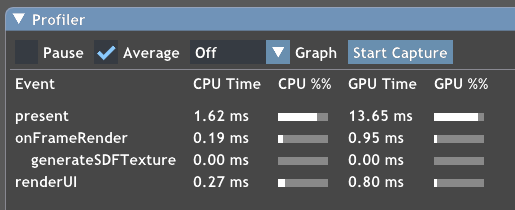
\includegraphics[width=0.4\textwidth]{gui/profiler.png}
	\caption{Profilozó ablak}
	\label{fig:profilerp}
\end{figure}

\subsection{Beállítások}

A felhasználói felület részeként a képernyő bal oldalán a jelenet és a generálás paraméterei találhatók. A beállításokat több lenyitható menübe szerveztem. A felületen találhatók gombok, számbeviteli mezők, csúszkák és lenyíló menük is, melyekkel több opció közül választhatunk. A számbeviteli mezőkbe dupla kattintással gépelni is lehet, illetve ha a bal egérgombot lenyomva oldalra húzzuk őket, akkor az érték nőni, illetve csökkeni fog előre beállítot határok között.

Figyelem, nem minden beállítás eredményez szép képet és helyes megjelenítést. Mivel a program célja a paraméterek beállítása, ez nem hibás működés.

\Aref{fig:global-settings} ábrán a globális beállítások találhatók. A Time mező az eltelt időt mutatja. A Scale paraméterrel beállíthatjuk, milyen gyorsan teljen. Alatta a felbontás állítható be. Ezt számbeviteli mezőkkel és legördülő menüből is kiválaszthatjuk. Készíthetünk még képernyőképet és videófelvételt is.

\begin{figure}[H]
	\centering
	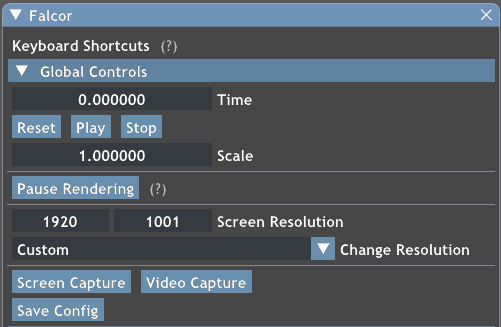
\includegraphics[width=0.4\textwidth]{gui/global.png}
	\caption{Globális beállítások}
	\label{fig:global-settings}
\end{figure}

\Aref{fig:camera-settings} ábrán a kamera beállításai szerepelnek. Az első paraméter a kamera mozgásának sebessége. A többi egy valódi kamera működését hivatott szimulálni. A Depth Range paraméter a közeli és távoli vágósík távolságát adja meg. Utána a kamera pozíciója és orientációja állítható be. Ezeket a paramétereket legkönnyebben a kamerát mozgató billentyűkkel és az egér mozgatásával állíthatjuk.

\begin{figure}[H]
	\centering
	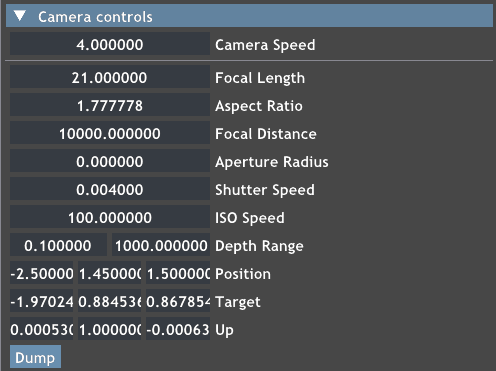
\includegraphics[width=0.4\textwidth]{gui/camera.png}
	\caption{Kamera beállítások}
	\label{fig:camera-settings}
\end{figure}

\Aref{fig:compute-settings} ábrán a felület generálásakor használt paramétereket lehet beállítani. Választhatunk a raszterizáció és a sugárkövetés között, vagy akár egymásra rajzoltathatjuk mindkettőt is. A ,,Generate new surface'' gombbal egy új felületet generálhatunk. A felület kontrollponthálóját az alatta lévő számbeviteli mezőkkel is állíthatjuk. A következő beállítások a távolságmező felbontása és a használt GPU oldali adatreprezentáció, mely minden generálási módszert érint. Az utolsó beállítás a generálási módszer, majd esetleg a módszer hiperparaméterei. Ezek sorban:
\begin{itemize}
	\item Lipschitz constant: a Lipschitz-módszer konstansa. Minél nagyobb, annál lassabb lesz a sugárkövetés. Ha túl kicsire állítjuk, a módszer nem konvergál.
	\item Number of iterations: az AdaMax módszer iterációszáma.
	\item Alpha, Beta1, Beta2: Az AdaMax módszer hiperparaméterei. A képminőséget csak extremális esetben vagy alacsony iterációszámnál befolyásolják.
\end{itemize}

\begin{figure}[H]
	\centering
	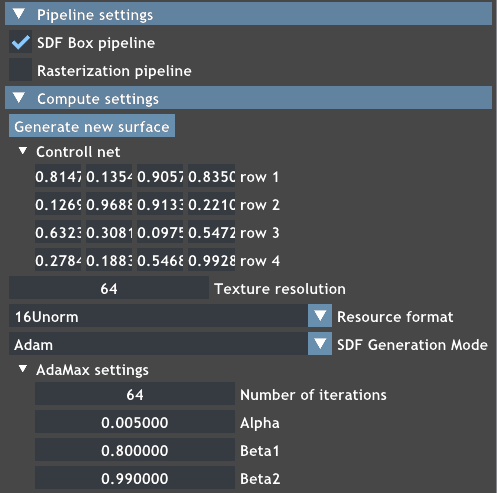
\includegraphics[width=0.4\textwidth]{gui/compute.png}
	\caption{Távolságmező-számításának beállításai}
	\label{fig:compute-settings}
\end{figure}

\Aref{fig:trace-settings} ábrán a sugárkövetés, fények és az anyagtulajdonság beállításai szerepelnek. A sugárkövetésnél beállítható a maximális iterációszám, a kilépési feltétel (Epsilon) és egy relaxációs paraméter, mellyel a sugárkövetés sebességét változtathatjuk. Figyelem, egynél nagyobb relaxációs értékekre nem garantált a konvergencia.

Beállítható egy ambiens fény, mely a tér minden pontját egyenlően megvilágítja. Egy csúszkával pontfényforrások adhatók a jelenethez, melyeknek a pozíciója és színe külön-külön állítható. A fényforrásoknak van egy alapbeállítása.

Az anyag tulajdonságai az alapszíne (Ambient), illetve a rajta látható visszaverődés diffúz és spakuláris komponenseinek erőssége. Az anyagtulajdonságokat szürkeárnyalatos és RGB formátumban is állíthatjuk.

\begin{figure}[H]
	\centering
	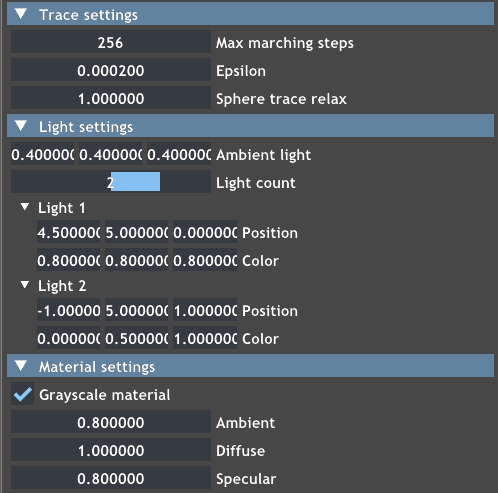
\includegraphics[width=0.4\textwidth]{gui/trace.png}
	\caption{Sugárkövetés, fények és anyagtulajdonság beállításai}
	\label{fig:trace-settings}
\end{figure}

\Aref{fig:box-settings} ábrán látható menüben a kirajzolt felületek pozíciója és mérete állítható.

\begin{figure}[H]
	\centering
	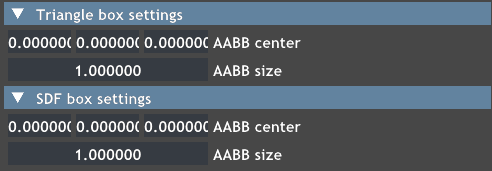
\includegraphics[width=0.4\textwidth]{gui/box.png}
	\caption{A kirajzolt dobozok pozíciója és mérete}
	\label{fig:box-settings}
\end{figure}

\section{Program futtatása}

A program futtatásához az alábbiak szükségesek: 
\begin{itemize}
	\item Windows 10
	\item GPU és DirectX 12 Driver
\end{itemize}
A futtatható állomány: \codeword{Falcor\build\windows-vs2019-d3d12\bin\Release\SDFBox.exe}


